\section{OpenTuner} \label{sec:ot}

OpenTuner search spaces are defined by \emph{Configuration}s, that are composed
of \emph{Parameter}s of various types. Each type has restricted bounds and
manipulation functions that enable the exploration of the search space.
OpenTuner implements ensembles of optimization techniques that
perform well in different problem domains. The framework uses
\emph{meta-techniques} to coordinate the distribution of resources
between techniques.
Results found during search are shared through a
database. An OpenTuner application can implement its own search
techniques and meta-techniques, making the ensemble more robust.
OpenTuner's source code is available\footnote{Hosted at GitHub:
\texttt{\scriptsize github.com/jansel/opentuner} [Accessed on 23 December 2015]} under the MIT License.

\begin{figure}[htpb]
    \centering
    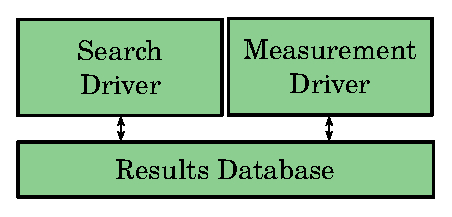
\includegraphics[scale=.62]{opentuner-implementation}
    \caption{Simplified OpenTuner Architecture.}
    \label{fig:ot-imp}
\end{figure}

Figure~\ref{fig:ot-imp} shows a high-level view of OpenTuner's architecture.
Measurement and searching are done in separate modules, whose main classes are
called \emph{drivers}. The search driver requests measurements by registering
configurations to the database. The measurement driver reads those
configurations and writes back the desired results. Using the measurement
driver available in the framework, the measurements are performed sequentially.

Before running the user-defined measurement function the OpenTuner measurement
% Não há necessidade de vírgula após "function" neste caso.
driver calls compilation hooks that can be run in parallel using Python
threads. When the autotuned program needs to be compiled only once, as in the
Travelling Salesperson example shown in Section~\ref{sec:exp}, the autotuner
could respond to more simultaneous result requests if the measurement driver
was able to also parallelize the runs of the user-defined measurement function.
% Aqui é "was" mesmo, pois concorda com o "could".

OpenTuner implements optimization techniques such as the
Nelder-Mead~\cite{nelder1965simplex} simplex method and Simulated
Annealing~\cite{kirkpatrick1983optimization}. A resource sharing mechanism,
called \emph{meta-technique}, aims to take advantage of the strengths of each
technique by balancing the exploitation of a technique that has produced good
results in the past and the exploration of unused and possibly better ones.
